
%(BEGIN_QUESTION)
% Copyright 2012, Tony R. Kuphaldt, released under the Creative Commons Attribution License (v 1.0)
% This means you may do almost anything with this work of mine, so long as you give me proper credit

A newly-installed {\sl Wireless}HART temperature transmitter (TT-34) located far away from the Gateway or any other {\sl Wireless}HART devices is having difficulty communicating with the Gateway because of the effect of distance on signal strength.  The pathway between TT-34 and the Gateway is free from obstructions.  One solution to this problem would be to install more {\sl Wireless}HART devices in between it and the Gateway to serve as signal repeaters, but unfortunately you do not have the time to order and install more devices -- this facility needs a solution and it needs one {\it now}:

$$\includegraphics[width=15.5cm]{i01223x01.eps}$$

Describe one solution which would work to improve TT-34's communication, which you could implement without ordering any new radio components (e.g. new antennas, more {\sl Wireless}HART devices, etc.).

\underbar{file i01223}
%(END_QUESTION)





%(BEGIN_ANSWER)

Full credit should be given for answers such as these:

\begin{itemize}
\item{} Placing a sheet metal ``reflector'' to the left of TT-34's antenna to make the antenna more directional and thereby improve its gain.
\item{} Relocating TT-34 to a higher location (this involves extending the RTD wires to that the RTD sensor may remain in the same location)
\item{} Relocating the Gateway closer to TT-34 (this involves extending the Ethernet cabling, which is generally very practical to do)
\end{itemize}

\vskip 10pt

Half credit should be given for less-than-practical solutions:

\begin{itemize}
\item{} Relocating TT-34 to a place closer to the Gateway (this would involve extending the RTD wiring a {\it long} way, since gains realized by reduced distance pale in comparison to gains realized by increased height)
\end{itemize}

%(END_ANSWER)





%(BEGIN_NOTES)

{\bf This question is intended for exams only and not worksheets!}

%(END_NOTES)


